\documentclass{article}
\usepackage[utf8]{inputenc}
\usepackage{graphicx}
\usepackage{minted}
\usepackage{hyperref}
\usepackage{textcomp}
\usepackage[dvipsnames]{xcolor}
\usepackage{comment}

\title{B-L072Z-LRWAN1 AT command}
\author{cmonaton }
\date{July 2019}

\begin{document}

\maketitle

\section{Introduction}
But : Se connecter à la carte B-L072Z-LRWAN1 et communiquer avec des commandes type AT. \\

\begin{figure}[H]
\begin{center}
\advance\leftskip-3cm
\advance\rightskip-3cm
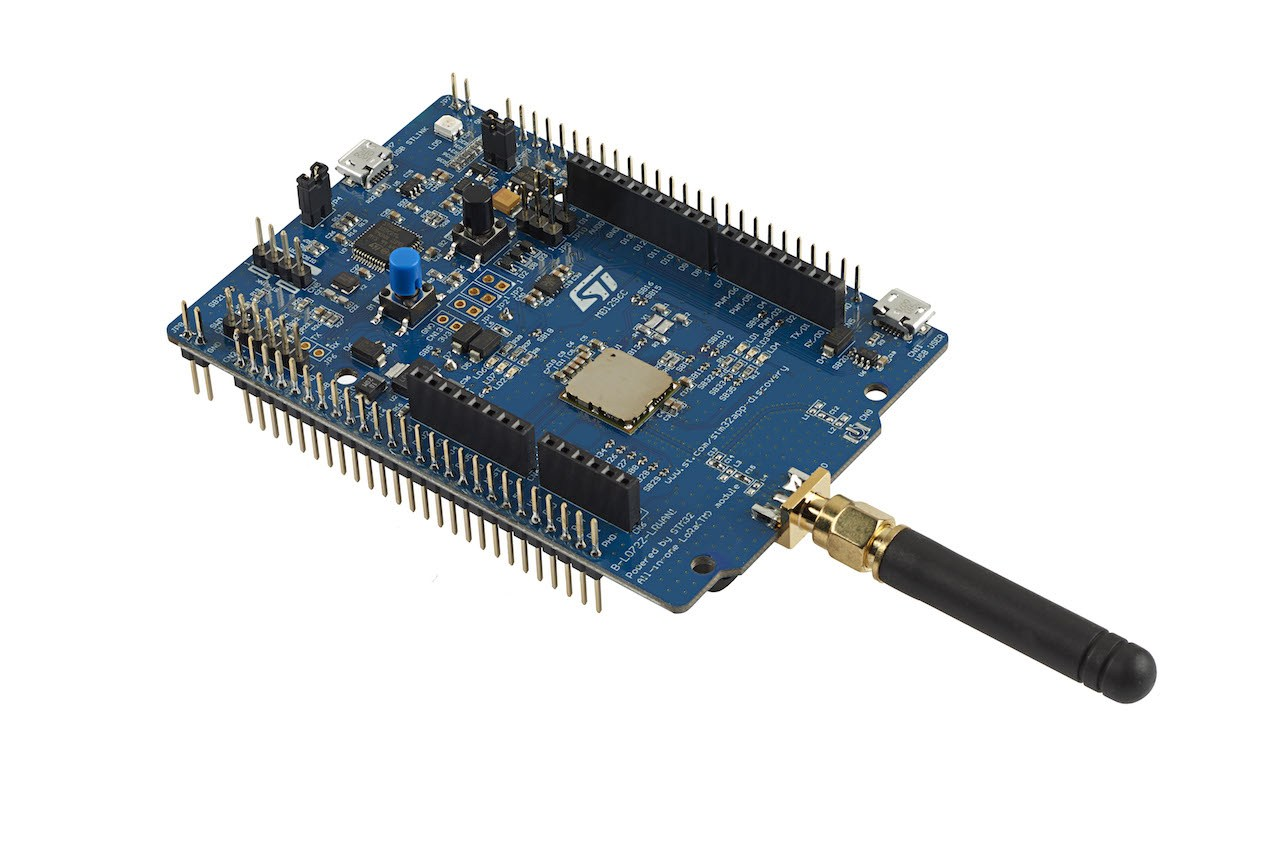
\includegraphics[keepaspectratio=true,scale=0.5]{carte.jpeg}
\label{visina8}
\end{center}\end{figure}


Projet AT\_Slave, le code se télécharge à  \url{https://www.st.com/en/embedded-software/i-cube-lrwan.html}

Prérequis : Flasher le code sur la carte et télécharger l'application AT\_Slave cf tuto \textit{B-L072Z-LRWAN1}


\begin{comment}
Pour : \begin{itemize}
    \item Télécharger le projet 
    \item télécharger du code sur la carte
    \item enregistrer la carte sur loraserver et recevoir les données
\end{itemize}
voir le tuto \textit{B-L072Z-LRWAN1}
\end{comment}

 \section{Matériel}
%carte : B-L072Z-LRWAN1


\textcolor{red}{Branchez l'antenne LoRa avant d'alimenter la carte sinon la carte grille}


\section{Commandes AT}

La liste des commade se trouve dans le fichier at.h \\

Emplacement :
\begin{minted}{bash}
/path_to_folder/STM32CubeExpansion_LRWAN_V1.2.1/Projects/B-L072Z-LRWAN1/
Applications/LoRa/AT_Slave/LoRaWAN/App/inc/at.h
\end{minted}





\begin{minted}{bash}
/* AT Command strings. Commands start with AT */
#define AT_RESET      "Z"
#define AT_DEUI       "+DEUI"
#define AT_DADDR      "+DADDR"
#define AT_APPKEY     "+APPKEY"
#define AT_NWKSKEY    "+NWKSKEY"
#define AT_APPSKEY    "+APPSKEY"
#define AT_JOINEUI     "+APPEUI" 
#define AT_ADR        "+ADR"
#define AT_TXP        "+TXP"
#define AT_DR         "+DR"
#define AT_DCS        "+DCS"
#define AT_PNM        "+PNM"
#define AT_RX2FQ      "+RX2FQ"
#define AT_RX2DR      "+RX2DR"
#define AT_RX1DL      "+RX1DL"
#define AT_RX2DL      "+RX2DL"
#define AT_JN1DL      "+JN1DL"
#define AT_JN2DL      "+JN2DL"
#define AT_NJM        "+NJM"
#define AT_NWKID      "+NWKID"
#define AT_FCU        "+FCU"
#define AT_FCD        "+FCD"
#define AT_CLASS      "+CLASS"
#define AT_JOIN       "+JOIN"
#define AT_NJS        "+NJS"
#define AT_SENDB      "+SENDB"
#define AT_SEND       "+SEND"
#define AT_RECVB      "+RECVB"
#define AT_RECV       "+RECV"
#define AT_VER        "+VER"
#define AT_CFM        "+CFM"
#define AT_CFS        "+CFS"
#define AT_SNR        "+SNR"
#define AT_RSSI       "+RSSI"
#define AT_BAT        "+BAT"
#define AT_TRSSI      "+TRSSI"
#define AT_TTONE      "+TTONE"
#define AT_TTLRA      "+TTLRA"
#define AT_TRLRA      "+TRLRA"
#define AT_TCONF      "+TCONF"
#define AT_TOFF       "+TOFF"
#define AT_CERTIF     "+CERTIF"
#define AT_PGSLOT     "+PGSLOT" 
#define AT_BFREQ      "+BFREQ"
#define AT_BTIME      "+BTIME"
#define AT_BGW        "+BGW" 
#define AT_LTIME      "+LTIME" 
\end{minted}

Après avoir téléchargé le code sur la carte, ouvrir putty ou minicom avec un baudrate de 9600 pour communiquer avec la carte. \\

\subsubsection{Pour ouvrir les ports ttyACM0 et ttyACM1 }

\textbf{Solution temporaire} 


\begin{minted}{bash}
sudo chmod 666 /dev/ttyACM0
\end{minted}
Il faut le entrez cette commande souvent. \\
\textbf{Solution permanente}\\

Créer un fichier dans son home

\begin{minted}{bash}
50-myusb.rules
\end{minted} 

l'éditer : 

\begin{minted}{bash}
KERNEL=="ttyACM[0-9]*",MODE="0666"
\end{minted}

Puis copiez ce fichier dans /etc/udev/rules.d/ et redémarrez votre PC. \\

\begin{minted}{bash}
 sudo cp 50-myusb.rules /etc/udev/rules.d
\end{minted}
C'est suffisant pour ne plus avoir à réouvrir les ports manuellement. Cependant, n'importe quel dispositif usb connecté au PC a maintenant le droit d'écriture sur le PC. \\

Pour plus de sécurité ajouter ces lignes dans ce fichier :

\begin{minted}{bash}
ACTION=="add", KERNEL=="ttyACM[0-9]*", ATTRS{idVendor}=="xxxx", 
ATTRS{idProduct}=="yyyy", MODE="0666"
\end{minted}
 
 Pour déterminer idVendor et idProduct des cartes tapez lsusb avant et après avoir connecter la carte. \\

 Dans mon cas avant et après avoir branché une carte externe :
 
 \begin{figure}[H]
\begin{center}
\advance\leftskip-3cm
\advance\rightskip-3cm
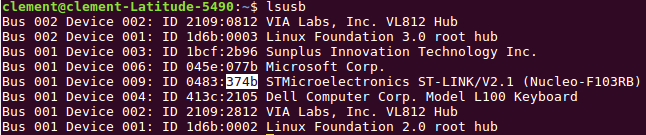
\includegraphics[keepaspectratio=true,scale=0.5]{lsusb.png}
\label{visina8}
\end{center}\end{figure}

idProduct = 374b\\
idVendor= 0483\\

Pour ajouter d'autres appareils, copier coller ces lignes en changeant idProduct et idVendor. \\

\section{Résultat}


%\begin{minted}{bash}
%sudo chmod 666 /dev/ttyACM0
%\end{minted}





\begin{figure}[H]
\begin{center}
\advance\leftskip-3cm
\advance\rightskip-3cm
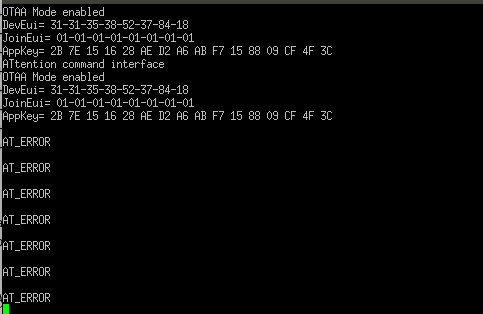
\includegraphics[keepaspectratio=true,scale=0.6]{putty.png}
\label{visina8}
\end{center}\end{figure}

Tapez les commandes même si rien ne s'affiche, c'est normal.

La commande \textit{ATZ} fonctionne bien.
Les autres semblent ne pas fonctionner.
\textit{AT} renvoie \textit{OK}

\end{document}
